\documentclass[letterpaper]{article}
\usepackage{config_flash}

\begin{document}

\section*{Programming Configuration Flash}
The FPGA's configuration is volatile, meaning it is lost when it loses power.
Flash devices on the other hand are non-volatile, so they will keep their stored files even
without power.
The Nexys4 board has a flash memory onboard that we can use to store the FPGA configuration file.
We can set the FPGA to load the configuration from flash when it is powered on.
These instructions are for Vivado 2018.2 but the steps are nearly the same in versions as
early as 2016.2.

The first thing we have to do is tell Vivado to generate a bin file during the Generate
Bitstream step. Right-click on PROGRAM AND DEBUG and select Bitstream Settings...

\arrowimage[0.8]{open_bitstream_settings}{{down,0.38,0.18},{down,0.75,0.16}}

In the window that pops up select the bin\_file option and press OK.

\arrowimage[1]{bitstream_settings}{{left,0.8,0.558},{down,0.557,0.06}}

Now run Generate Bitstream, this time a .bin file will be generated.
Then open the Hardware Manager either by clicking Open Hardware Manager under the PROGRAM
AND DEBUG section or if a window pops up when generating bitstream is complete select Open
Hardware Manager.

\arrowimage{bitstream_complete}{{left,0.54,0.47},{down,0.6,0.12}}

Now open the hardware target.

\arrowimage[1]{open_target}{{left,0.77,0.633},{left,0.83,0.53}}

The option to Add Configuration Memory Device is now available, click it.
A context menu will pop up with the FPGA as the only option to add a memory device to, click it.

\arrowimage[1]{add_config_memory_device}{{down,0.35,0.099},{left,0.56,0.045}}

The flash part has to be selected.
The Nexys 4 and Nexys 4 DDR both have a Spansion s25fl128s Quad SPI Flash.
If you are programming a Nexys 4 or Nexys 4 DDR your selection should be as shown below.

\arrowimage[1]{select_part_nexys4}{{down,0.25,0.65},{down,0.32,0.18},{down,0.833,0.07}}

The Basis 3 has a Spansion s25fl032p Quad SPI Flash, shown below.
If you are programming a Basys 3 your selection should be as shown below.

\arrowimage[1]{select_part_basys3}{{down,0.31,0.65},{down,0.33,0.23},{down,0.776,0.08}}

After selecting the part a window will pop up asking to program the memory now.
Press OK.

\arrowimage[1]{program_now}{{down,0.671,0.25},}

The default programming options should be OK, but make sure they match here.
This will erase the flash, program the new configuration, and verify that it programmed correctly.
Also verify that the .bin file is correct, then press OK to program.

\arrowimage[1]{program}{{right,0.41,0.056},}

To load the FPGA configuration from the Quad SPI Flash, the configuration jumpers must be
set correctly.
For the Nexys 4 and Nexys 4 DDR use the following settings.

\begin{center}
    \begin{tikzpicture}[box/.style={line width=4pt, darkred!70}]
    \node[anchor=south west,inner sep=0] (image) at (0,0)
    {
        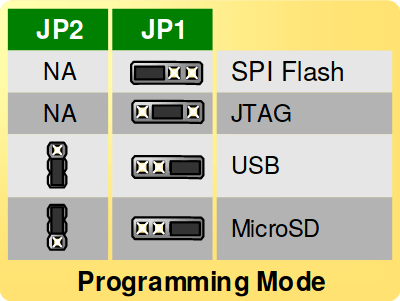
\includegraphics[width=0.5\textwidth]{jumpers_nexys4}
    };
    \begin{scope}[x={(image.south east)},y={(image.north west)}]
        \draw[box] (0.02,0.69) rectangle ++(0.96,0.14);
    \end{scope}
    \end{tikzpicture}
\end{center}

For the Basys 3 use the following jumper settings.

\begin{center}
    \begin{tikzpicture}[box/.style={line width=4pt, darkred!70}]
    \node[anchor=south west,inner sep=0] (image) at (0,0)
    {
        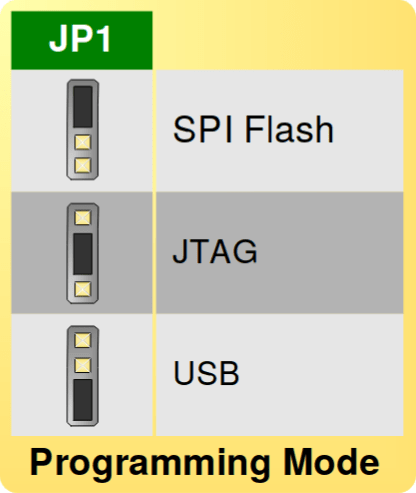
\includegraphics[width=0.5\textwidth]{jumpers_basys3}
    };
    \begin{scope}[x={(image.south east)},y={(image.north west)}]
        \draw[box] (0.02,0.61) rectangle ++(0.96,0.25);
    \end{scope}
    \end{tikzpicture}
\end{center}

If you didn't select the correct jumper setting before programming, you will have to press
the prog button or power cycle the board to program the FPGA with the contents of the Flash.

\end{document}
